\documentclass[11pt]{article} 
\usepackage{geometry}
\usepackage[utf8]{inputenc}
\inputencoding{utf8}
\geometry{a4paper}
\usepackage{graphicx}
\usepackage[table,xcdraw]{xcolor}
\usepackage{pdfpages}
\usepackage{tabu}
\usepackage{longtable}

\graphicspath{{images/}}

\begin{document}

%----------------------------------------------------------------------------------------
%	TITLE PAGE
%----------------------------------------------------------------------------------------

\begin{titlepage}

\newcommand{\HRule}{\rule{\linewidth}{0.5mm}}
\center
\textsc{\LARGE King's College London}\\[1.5cm]
\textsc{\Large Traffic Simulator}\\[0.5cm]
\textsc{\large Group Project}\\[0.5cm]
\HRule \\[0.4cm]
{ \huge \bfseries Team Diversity}\\[0.4cm]
\HRule \\[1.5cm]

\begin{minipage}{0.4\textwidth} \large
\begin{center}
\emph{Members:}\\
Balázs Kiss \\
Eddy Mukasa \\
Yukolthep Visessmit \\
Pongsakorn Riyamongkol \\
Snorri Hannesson
\end{center}
\end{minipage}
\\[2cm]


\includegraphics{KingsLogo}\\[1cm] 

{\large \today}\\[3cm]

\vfill

\end{titlepage}

%----------------------------------------------------------------------------------------
%	Table of contents
%----------------------------------------------------------------------------------------

\tableofcontents

\newpage
%----------------------------------------------------------------------------------------
%	Introduction: Describe the context for the work and the problem you are addressing. Briefly summarise what you achieved in the project.
%----------------------------------------------------------------------------------------

\section{Introduction}
	\subsection{Background}
	\subsection{Descriptions: like a abstract}
	\subsection{Methodology} 
	\subsection{Theory}
	\subsection{Goal}
	\subsection{Scope}
	\subsection{Schedule: Chart + text explain}
	\subsection{Obstacle}
	\subsection{br sum => find word (about program) // no need bc 1.1-1.5 is br sum}
	
\newpage
%----------------------------------------------------------------------------------------
%	Related Work: Describe related work.
%----------------------------------------------------------------------------------------
\section{Related Work}
In today's world a lot of effort is made to make transportation as good as possible. For most countries and cities the road systems is a vital part of it's transportation system. With the ever growing population and increasing purchasing power of the public, good traffic control has never been as urgent. Changes to road systems are hard to make and drivers wouldn't be pleased if many experiments were made on live traffic. That's why traffic simulators play a big role in increasing the quality of the road system. Any change can be simulated and the result of the change can be analysed. There are many challenges that traffic simulation creators face. Trying to predict the behaviour of drivers and the synergistic effects of different factors can have on a driver behaviour is perhaps the most challenging, the goal is to make it as realistic as possible.\\

Many traffic simulators exist as well as many papers and books on that subject. In this module we were given two papers on traffic simulation for inspiration for this project and an insight into this field. Sewall, Wilkie, Merrell and Lin \cite{sewall2010continuum}presented a novel method for the synthesis and animation of realistic traffic flows on large-scale road networks. Their technique is based on a continuum model of traffic flow they extended to correctly handle lane changes and merges, as well as traffic behaviours due to changes in speed limit. They demonstrated how their method can be applied to the animation of many vehicles in a large-scale traffic network at interactive rates and showed that their method can simulate believable traffic flows on publicly available, real-world road data. They furthermore demonstrated the scalability of this technique on many-core systems.\\

Namekawa, F. Ueda, Hioki, Y. Ueda and Satoh \cite{namekawa2005general} spent several years developing a general purpose road-traffic simulation system to analyse road traffic jams. The concept of their system was using the running line model as opposed to fixed road-network information database, which is not effective in their opinion. Their simulator uses the a cell automaton model.


\newpage	
%----------------------------------------------------------------------------------------
%	Requirement and Design: Describe the requirements you set for your project at the beginning and the design you have taken for your project. Focus on why you decided to tackle the problem in the way you did, and what effects that had on the design. You may also wish to mention the impact of team-working on your requirements and design.
%----------------------------------------------------------------------------------------	
\section{Requirement and Design}
	\subsection{Requirement}
	\subsection{Design}
	
\newpage
%----------------------------------------------------------------------------------------
%	Implementation: Describe the most significant implementation details, focussing on those where unusual or detailed solutions were required. Quote code fragments wherenecessary, but remember that the full source code will be included as an appendix. Ex- plain how you tested your software (e.g. unit testing) and the extent to which you tested it. If relevant to your project, explain performance issues and how you tackled them.
%----------------------------------------------------------------------------------------
\section{Implementation}

\subsection{Maps}

Flexible model
\\
Map, Roads, Lanes, Junctions
\\
Class Diagram
\\
Usage examples

\subsection{Drivers \& Vehicles}

Separation of driver and vehicle, driver makes decisions
\\
Different driver classes
\\
Different vehicle classes

\subsection{Traffic Policies}

Traffic Lights
\\
Fixed time \& congestion policies

\subsection{Running the Simulation}

Simulation class and subclasses
\\
ISteppable interface
\\
timing
\\
Generating cars
\\
Results

\subsection{Graphical User Interface}
In our application, JavaFX is selected as a graphic platform to be used. This platform allows developers to create an application on various platform such as desktop, mobile, or web. Furthermore, this platform introduce the use of cascading style sheets (CSS) to decorate the interface. This way, coders won’t have to worry about decorating the interface themselves in their codes and let CSS designer to handle this instead. Although in our application the use of this benefit haven’t been implemented along with the java code but we think that this is a very helpful technique worth mentioned from JavaFX.
Our application consists of 2 stages, which are both a top-level container of JavaFX, one is the main stage that will show a simulation and another one is the one used to show a simulation’s result. The first stage is separated into 2 parts by using Border pane. This pane works like BorderLayout in Javaswing but in JavaFX this layout is implemented into a pane rather than being one of the layout to be set into an empty pane. The followings are put into left and center region of this border pane respectively:
\subsubsection{Canvas}
Canvas is a node that is a blank image. This node can be painted on using GraphicsContext class object. Our canvas has a width of 800 pixels and height of 600 pixels so we don’t have to worry about how our application will run in different screen resolution since this dimension is probably comply with all present screen resolutions. To draw a simulation, we can call a GraphicsContext object from canvas itself using \texttt{getGraphicsContext2D()} and by doing so, we can manipulate the canvas with various methods from GraphicsContext like \texttt{fillPolygon(double[] X, double[] Y)} which will draw a polygon with specified fill colour from a set of coordinate X and Y. To draw roads, we can call an above method and get a set of parameters from a simulation class which contains a list of roads. Each road can provide its own coordinate at each corner so we use this as elements to be added into a set of X and Y coordinate. Because this is a “fill” type method which will also paint an enclosure of a polygon we can provide only 3 points to the method which these are \texttt{leftStartPoint},\texttt{leftEndPoint}, and \texttt{rightEndPoint}. The method automatically close the gap between a start point and last point with a straight line and fill a polygon afterwards. For vehicles, we have already provided a picture for each type of vehicle in a JPEG format and draw these pictures based on what type of vehicle we are dealing with from a list of vehicle provided from simulation class. There is a useful method in Vehicle class called \texttt{getDisplacementVector()}, using this method along with the one in Point class from utils package called \texttt{angleVectorDegree()} we obtain an angle in which a vehicle is running compare to a horizontal line measuring In counter-clockwise manner. After we obtained a value of angle, a method called \texttt{drawRotatedImage()} will do a job to draw a vehicle picture onto a canvas. This method, again, call another method \texttt{rotate()} which receive 4 parameters consist of GraphicsContext object, angle value, x-position, and y-position where these x and y form a coordinate in which will be an anchor point of the rotation. After that, we create a rotate class object by using above parameters. This rotate class object will perform a calculation in order to make a GraphicsContext rotate before we actually draw something using it. After we have rotated the GraphicsContext, we can normally draw a picture onto a canvas.
\subsubsection{Settings panel}
In this panel, we take an advantage from JavaFX features called HBox and VBox, which will place objects horizontally and vertically next to previous one by specified insets. The idea is to put many Hboxes into one VBox but since radio buttons still require us to put them in vertically, so we have put one VBox into Hbox to be able to put radio buttons in their correct position. Figure x given below will give an overall image of how we put each component together within this pane (HBox indicated by red border, VBox indicated by black border and object are indicated by blue green border).
\\
\begin{center}
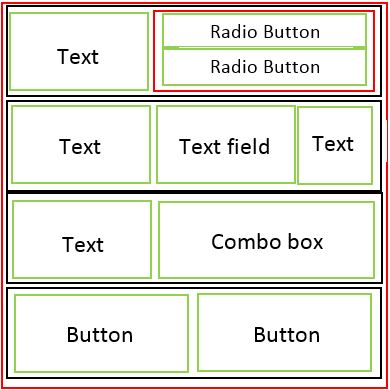
\includegraphics{GUI_component}\\
\textit{Figure x}
\end{center}

\newpage
%----------------------------------------------------------------------------------------
%	Team Work: Describe how you worked together, including the tools and processes you used to facilitate group work.
%----------------------------------------------------------------------------------------
\section{Team Work}
In this chapter we'll describe how we worked together during this project, including the tools and processes we used to facilitate group work. We'll will not reflect on what went wrong and what worked well, that is the focus of chapter 6 - Evaluation.
\subsection{Methodology}
A slightly adjusted Agile methodology was used for this project. What is meant be that is we did not follow Agile to the bone but we took bits and pieces from Agile that we knew from previous studies and work experience. The bits and pieces we chose to use from Agile are things that we believed would work for us in this project, i.e. iterations, user stories, roles and we used test driven development to some extend.
\subsubsection{Roles}
\textbf{Balázs Kiss:} Lead programmer\\
\textbf{Eddy Mukasa:} Architect \\
\textbf{Yukolthep Visessmit:} Graphical designer \\
\textbf{Pongsakorn N. Riyamongkol:} Project Manager \\
\textbf{Snorri Hannesson:} Tester and Coordinator \\ \newline
Each member of the group had a responsibility to oversee one aspect of the project but was not expected to do all the work defined in his role. I.e. each member should/could do some programming but the lead programmer should oversee the code and make sure nothing is missing and everything is done properly. The same goes for the other roles.

\subsection{Physical meetings}
Every Thursday at 10 o'clock we had a physical meetings where all team members were expected to attend. We kept log of our meetings so those who were unable to attend the meeting could get up to date by reading the log and for those who did attend the meeting to refresh their memory of what was discussed in the meeting.
In these meetings we discussed the progress we made from last meeting and the problems we were faced with. At the end of each meeting we allocated work to each member witch is supposed to be done during the week until next meeting.
Occasionally extra meetings have been scheduled where a certain aspect of the project been focused on. Not all members are expected to attend these meetings but only the members who are focusing on this certain aspect of the project.
\subsection{GitHub}
Github was used for version control. Our branching strategy was that every time a member wanted to implement a new feature to the system or write something to the report, a new branch was created for that feature. When that branch was created it would be up to date with the master. When work were done on that branch a pull request would be made to the master. The leader of that aspect of the project would then decide to merge or to create a new branch with suggestions of improvements or alterations. Those improvements could then be merged with the original branch which could then be merged with master.
\subsection{Facebook}
Facebook was used as a communication channel. The first thing this team did was to create a facebook group for the team. Most people these days use facebook everyday so this is very convenient communication channel. In this group we would have various discussions about the our progresses or problems. The facebook chat was also used for individual members to discuss matters that were not directly associated to the group as a whole but only the members in the chat.
\subsection{Trello}
Trello is a versatile tool which was used for project management. The rationale for using Trello is that it's very flexible so you can modify the interface to your will. In this project not all tasks were code related which is not a problem when using Trello. 


\newpage
%----------------------------------------------------------------------------------------
%	Evaluation: Critically evaluate your project: what worked well, and what didn’t? how did you do relative to your plan? what changes were the result of improved thinking and what changes were forced upon you? how did your team work together? etc. Note that you need to show that you understand the weaknesses in your work as well as its strengths. You may wish to identify relevant future work that could be done on your project.
%----------------------------------------------------------------------------------------
\section{Evaluation}

\newpage	
%----------------------------------------------------------------------------------------
%	Peer Assessment: In a simple table, allocate the 100 ‘points’ you are given to each team member. Valid values range from 0 to 100 inclusive. You may assign decimal values, but the entire points must add up to precisely 100.
%----------------------------------------------------------------------------------------
\section{Peer Assessment}

\indent\indent Robert T. \cite{roberts2006self} states that “The term peer assessment refers to the process of having the learners critically reflect upon, and perhaps suggest grades for, the learning of their peers.” In the other words, peer assessment is a process which student are able to assess their friends based on the criteria. This causes student to provide some feedbacks and evaluate their friends, which may help learning together (University of Reading, 2015). Therefore, TeamDiversity is going to use the peer assessment method for grading our member. This will be going to focus on the methodology which is used for assessment following by the criteria. It will be then shown the result and summary of each member in TeamDiversity. 
	\subsection{How do we evaluate our member?}
	
	\indent\indent I. Distribute the assessment form and assessment criteria to our member.\\
	\indent II. In each member, he/she must score himself/herself as well as other group member. For example, if our team has 4 people, it will grade 1 for yourself and 3 for our friends.\\
	\indent III. When you have completed a score (your friends and yourself), you need to mark total add up all scores and calculate the average score for yourself. \\
	\indent IV. We use only the average score to evaluate our friends and present in this report. 


	\subsection{What is the criteria that we have used?}
		\indent University of Sydney (2015) has published the assessment criteria and form on the website. TeamDiversity has adapted both documents in the appropriate way for supporting our task. This criteria is going to evaluate ten aspects of member behaviour. In each aspect, we have scored in the range from 0—10. Thus, the total marks of each member will vary from 0—100 inclusive. There will be then illustrated the detail in each aspect of peer assessment criteria, as followed \newline 

\textbf{A. Quantity of Work:}\\
	\indent\indent 0	- not taking part in it, having no prospect of progress/value \\
	\indent\indent 1—2	- doing a particular, not too much but enough\\
	\indent\indent 3—4	- sometimes above standard, generally needs improvement \\
	\indent\indent 5—6	- satisfactory, doing more than requirement \\
	\indent\indent 7—8	- always working hard and consistent \\
	\indent\indent 9—10	- outstanding, always over productivity standards \\

\textbf{B. Quality of Work:}\\
	\indent\indent 0	- not giving sufficient attention, making frequent mistakes\\
	\indent\indent 1—2	- giving attention, making some mistakes\\
	\indent\indent 3—4	- doing well, basically correct\\
	\indent\indent 5—6	- satisfactory, accurate in some aspect\\
	\indent\indent 7—8	- almost accurate in all involving fields\\
	\indent\indent 9—10	- outstanding, perfect work\\

\textbf{C. Communication Skills:}\\
	\indent\indent 0	- having bad manners, not showing respect for other people, not listen\\
	\indent\indent 1—2	- friendly and easy to talk to once know by others\\
	\indent\indent 3—4	- warm and friendly, sociable\\
	\indent\indent 5—6	- showing good manners, kindly, listens and understands\\
	\indent\indent 7—8	- courteous and respectful, best wish\\ 
	\indent\indent 9—10	- Inspiring to others, excellent at listening and understanding\\

\textbf{D. Initiative:}\\
	\indent\indent 0	- acts without plan/purpose\\
	\indent\indent 1—2	- need encouragement to do task\\
	\indent\indent 3—4	- putting in minimal effort to complete task\\
	\indent\indent 5—6	- desire to achieve task/goal\\
	\indent\indent 7—8	- strongly desire to achieve task/goal\\
	\indent\indent 9—10	- beyond duty, high motivation\\

\textbf{E. Efficiency:}\\
	\indent\indent 0	- always delayed\\
	\indent\indent 1—2	- occasionally finished on time\\  
	\indent\indent 3—4	- usually finished on time, having minor errors\\
	\indent\indent 5—6	- always finished on time\\
	\indent\indent 7—8	- absolutely completed, consistent in troubleshooting and solving major problems\\ 
	\indent\indent 9—10	- invariably completed ahead of schedule, showing creativity, making major contributions\\ 

\textbf{F. Personal Relations:}\\
	\indent\indent 0	- very disruptive influence\\
	\indent\indent 1—2	- some friction\\
	\indent\indent 3—4	- no problem, commonly\\
	\indent\indent 5—6	- satisfactory, tuneful, harmonious\\ 
	\indent\indent 7—8	- positive factor\\
	\indent\indent 9—10	- respect by others\\

\textbf{G. Group Meeting Attendance:}\\
	\indent\indent 0	- never attended to meeting, not interest\\
	\indent\indent 1—2	- sometime attended \\
	\indent\indent 3—4	- usually attended, hard to get touch with\\
	\indent\indent 5—6	- attend, normally late\\
	\indent\indent 7—8	- count on to attend\\
	\indent\indent 9—10	- never ever missed a meeting, on time\\

\textbf{H. Attitude and Enthusiasm:}\\
	\indent\indent 0	- low disposition, having no prospect of value, unconcerned \\
	\indent\indent 1—2	- feeling/showing few excitement, blasé\\
	\indent\indent 3—4	- half hearted \\
	\indent\indent 5—6	- positive outward behaviour/bearing\\
	\indent\indent 7—8	- positive attitude and spirited\\
	\indent\indent 9—10	- excitement and eager, inspiring to others, positive thinking and influence\\

\textbf{I. Effort:}\\
	\indent\indent 0	- expects others to carry the load\\
	\indent\indent 1—2	- leave some effort\\
	\indent\indent 3—4	- displays enough endeavour\\
	\indent\indent 5—6	- firm and stable contributions\\
	\indent\indent 7—8	- energetic\\
	\indent\indent 9—10	- self starter, normally beyond duty\\

\textbf{J. Dependability:}\\ 
	\indent\indent 0	- unreliable\\
	\indent\indent 1—2	- unsteady, but slightly dependability \\
	\indent\indent 3—4	- inconsistent, occasionally be\\
	\indent\indent 5—6	- suitable, need some improvement \\
	\indent\indent 7—8	- very trustworthy, responsibility \\
	\indent\indent 9—10	- always responsible, steady influence \\
	\subsection{What is there result and summary of peer assessment?}

\newpage	
%----------------------------------------------------------------------------------------
%	References
%----------------------------------------------------------------------------------------
\bibliographystyle{plain}
\bibliography{References}


\newpage	
%----------------------------------------------------------------------------------------
%	Appendices
%----------------------------------------------------------------------------------------
\addtocontents{toc}{\vspace{2em}}

\appendix
% Appendix A: the Gitlog

\section{Gitlog}
\label{AppendixA}

\begin{center}
\begin{longtabu} to \textwidth {|
    X[4,l]|
    X[3,c]|
    X[8,l]|}
    \hline
    \textbf{Author} & \textbf{Date} & \textbf{Message} \\ \hline
Balázs Kiss & 2015-01-25 & Initial architecture \\ \hline
Balázs Kiss & 2015-01-26 & Ignore build directory \\ \hline
snh11 & 2015-01-26 & Meeting log created, first three meetings documented \\ \hline
Snorrihann & 2015-01-26 & A template for the initial report \\ \hline
Snorrihann & 2015-01-28 & More work done on the intital report \\ \hline
Snorrihann & 2015-01-29 & Modification of roles \\ \hline
Snorrihann & 2015-01-29 & sdfsf dfsd ds \\ \hline
Snorrihann & 2015-01-29 & Change to conflicts \\ \hline
Snorri Hannesson & 2015-01-29 & Merge pull request \#1 from teamDiversity/Snorri\_Conflicts \\ \hline
Balázs Kiss & 2015-02-01 & Speed model for vehicles, basic collison avoidance \\ \hline
Balázs Kiss & 2015-02-01 & Merge pull request \#2 from teamDiversity/develop\_speed \\ \hline
Snorrihann & 2015-02-03 & meeting 29th of january \\ \hline
Snorri Hannesson & 2015-02-03 & Merge pull request \#3 from teamDiversity/meeting\_log \\ \hline
Snorrihann & 2015-02-04 & Implementation of different types of vehicles \\ \hline
Snorrihann & 2015-02-04 & Changes on the initial report made by Neab \\ \hline
Snorri Hannesson & 2015-02-04 & Merge pull request \#4 from teamDiversity/initialReport\_NeabChanges \\ \hline
Snorri Hannesson & 2015-02-04 & Update .gitignore \\ \hline
Snorri Hannesson & 2015-02-04 & Delete initialReport.txt \\ \hline
Snorri Hannesson & 2015-02-04 & Delete initialReport.wc \\ \hline
Balázs Kiss & 2015-02-05 & Corrected my name \\ \hline
Balázs Kiss & 2015-02-05 & Merge pull request \#5 from teamDiversity/report\_typo \\ \hline
Balázs Kiss & 2015-02-05 & Removed junk \\ \hline
Balázs Kiss & 2015-02-05 & Merge pull request \#6 from teamDiversity/report\_typo \\ \hline
Balázs Kiss & 2015-02-05 & Moved vehicle classes to separate package \\ \hline
Balázs Kiss & 2015-02-05 & Use protected topSpeed field for vehicles \\ \hline
Snorrihann & 2015-02-05 & Merge branch `develop\_carsAndBuses\_improvements' of https://github.com/teamDiversity/trafficSim \\ \hline
Snorrihann & 2015-02-05 & Succestions of improvements implemented \\ \hline
yukolthep & 2015-02-05 & first gui implementation \\ \hline
Balázs Kiss & 2015-02-05 & Merge pull request \#9 from teamDiversity/master \\ \hline
Snorrihann & 2015-02-05 & meeting 5th of feb \\ \hline
Snorri Hannesson & 2015-02-05 & Merge pull request \#7 from teamDiversity/develop\_carsAndBuses\_improvements \\ \hline
Snorri Hannesson & 2015-02-05 & Merge pull request \#10 from teamDiversity/develop\_carsAndBuses \\ \hline
Snorrihann & 2015-02-05 & Merge branch `master' of https://github.com/teamDiversity/trafficSim \\ \hline
Snorrihann & 2015-02-05 & acceleration re-changed to maxAcceleration \\ \hline
Snorri Hannesson & 2015-02-05 & Merge pull request \#11 from teamDiversity/development\_maxAcceleration \\ \hline
Snorrihann & 2015-02-05 & Meeting 5th feb logged \\ \hline
Snorri Hannesson & 2015-02-05 & Merge pull request \#13 from teamDiversity/meeting\_5thFeb \\ \hline
Snorrihann & 2015-02-05 & The mandatory/optional table and some proofreading \\ \hline
Balázs Kiss & 2015-02-07 & These files were not the latest \\ \hline
Balázs Kiss & 2015-02-07 & Merge branch `master' into gabb\_branch\_merge \\ \hline
Balázs Kiss & 2015-02-07 & put back maxAcceleration \\ \hline
Balázs Kiss & 2015-02-07 & Merged vehicle subclasses \\ \hline
Balázs Kiss & 2015-02-07 & Changed project type to Java FX \\ \hline
Balázs Kiss & 2015-02-07 & Cleanup \\ \hline
Balázs Kiss & 2015-02-07 & Merge pull request \#14 from teamDiversity/gabb\_branch\_merge \\ \hline
Balázs Kiss & 2015-02-07 & Simulation classes \\ \hline
Balázs Kiss & 2015-02-07 & Removed unnecessary parts from GUISimulation class \\ \hline
Balázs Kiss & 2015-02-07 & Merge pull request \#15 from teamDiversity/simulation\_classes \\ \hline
Balázs Kiss & 2015-02-07 & Small changes \\ \hline
Balázs Kiss & 2015-02-07 & Merge pull request \#16 from teamDiversity/initial\_report\_balazs \\ \hline
Pongsakorn N. Riyamongkol & 2015-02-08 & 1. This is the same as InitialReport.tex 2. If i edit, it is in this pool 3. I will put presentation slide too \\ \hline
Snorrihann & 2015-02-09 & Changes made on the meeting 9 feb \\ \hline
Snorri Hannesson & 2015-02-09 & Merge pull request \#17 from teamDiversity/intialReport\_changesFromMeeting9Feb \\ \hline
Snorrihann & 2015-02-09 & Meeting log 9th of feb \\ \hline
Snorrihann & 2015-02-09 & Changes made to fit requirements on the `Nodes on the inital report' \\ \hline
Snorri Hannesson & 2015-02-09 & Merge pull request \#18 from teamDiversity/meeting\_9thFeb \\ \hline
Snorri Hannesson & 2015-02-09 & Merge pull request \#19 from teamDiversity/intialReport\_changesFromMeeting9Feb \\ \hline
eddymukasa & 2015-02-10 & UML Use case and Class diagram \\ \hline
eddymukasa & 2015-02-10 & Updates to UML Class multiplicities \\ \hline
eddymukasa & 2015-02-10 & Merge pull request \#20 from teamDiversity/UMLDesigns \\ \hline
eddymukasa & 2015-02-10 & Updates to UML Class multiplicities \\ \hline
eddymukasa & 2015-02-10 & merge conflict resolution \\ \hline
eddymukasa & 2015-02-10 & new class diagram \\ \hline
yukolthep & 2015-02-11 & update on car's picture \\ \hline
Balázs Kiss & 2015-02-11 & Merge branch `UMLDesigns' \\ \hline
Balázs Kiss & 2015-02-11 & Merge branch `master' into develop\_gui \\ \hline
Balázs Kiss & 2015-02-11 & Renderer classes, code cleanup \\ \hline
Balázs Kiss & 2015-02-11 & Fixed thread synch bug \\ \hline
Balázs Kiss & 2015-02-11 & Better map for testing \\ \hline
Snorrihann & 2015-02-12 & First tests, just for fun \\ \hline
Snorri Hannesson & 2015-02-12 & Merge pull request \#22 from teamDiversity/test\_basicInitialTestSuite \\ \hline
yukolthep & 2015-02-16 & draw horizontal and vertical roads, still rotated road left \\ \hline
Snorrihann & 2015-02-18 & More tests on vehicle and road system and a test suite class created \\ \hline
Snorri Hannesson & 2015-02-18 & Merge pull request \#23 from teamDiversity/test\_basicFunctions \\ \hline
Snorrihann & 2015-02-18 & jUnit library added to project.properties \\ \hline
Snorrihann & 2015-02-18 & jUnit library added to project.properties \\ \hline
Snorrihann & 2015-02-18 & meeting log updated \\ \hline
Snorri Hannesson & 2015-02-18 & Merge pull request \#25 from teamDiversity/meeting\_11feb \\ \hline
Snorrihann & 2015-02-19 & First creation of final report \\ \hline
Snorri Hannesson & 2015-02-19 & Merge pull request \#26 from teamDiversity/finalReport\_SnorriInitialWork \\ \hline
Snorri Hannesson & 2015-02-19 & Merge pull request \#24 from teamDiversity/test\_jUnitLibrary \\ \hline
Snorrihann & 2015-02-19 & meeting 19feb \\ \hline
Snorri Hannesson & 2015-02-19 & Merge pull request \#27 from teamDiversity/meeting\_19feb \\ \hline
yukolthep & 2015-02-19 & try some manual drawing. still have problem with wrong drawing of rotated road. The angle calculated using the formula seems to be correct but after draw the rotated rectangular with specified angle, it is not correct as the road is drawn with wrong angle. Still can't figure out what is the cause. \\ \hline
eddymukasa & 2015-02-19 & Adding driver Classes to project \\ \hline
eddymukasa & 2015-02-19 & CautiousDriver fix \\ \hline
yukolthep & 2015-02-20 & - fix drawVehicle to correctly draw car using correct angle. - Simulation2 class is used for testing different rotated roads drawing \\ \hline
Snorrihann & 2015-02-20 & Roads and lanes now have four points as a paramiter: leftStart, rightStart, leftEnd, rightEnd. Roads are initialised by the leftStart and leftEnd. \\ \hline
Balázs Kiss & 2015-02-21 & Project properties \\ \hline
Balázs Kiss & 2015-02-21 & step counter \\ \hline
Balázs Kiss & 2015-02-21 & Removed vehicle position from constructor \\ \hline
Balázs Kiss & 2015-02-21 & inherited type method \\ \hline
Balázs Kiss & 2015-02-21 & Removed lane from constructor \\ \hline
Balázs Kiss & 2015-02-21 & Removed unneded methods \\ \hline
Balázs Kiss & 2015-02-21 & Vehicles added at entrypoint \\ \hline
Balázs Kiss & 2015-02-21 & vehicles exit the system \\ \hline
Balázs Kiss & 2015-02-21 & Simualtion stops when all cars exited the system \\ \hline
Balázs Kiss & 2015-02-21 & Passing tests \\ \hline
Balázs Kiss & 2015-02-21 & Merge pull request \#28 from teamDiversity/entry\_and\_exit\_points \\ \hline
Balázs Kiss & 2015-02-21 & Merge development\_widthOfLanes \\ \hline
Balázs Kiss & 2015-02-21 & Merge development\_widthOfLanes \\ \hline
Balázs Kiss & 2015-02-22 & Merge branch `development\_widthOfLanes' \\ \hline
yukolthep & 2015-02-23 & - added new simple car and bus image. - draw vehicles based on their type. - fixed Normal and Cautious bus to extend from Bus class instead of Car class. \\ \hline
yukolthep & 2015-02-23 & - fixed using class instead of string to decide what type of vehicle it is \\ \hline
yukolthep & 2015-02-23 & - changed canvas size back to 800x600 \\ \hline
yukolthep & 2015-02-27 & - clean up some unused test code - bug in drawing a car with wrong position possibly caused by the position of vehicle itself as the position reading from a command line is wrong. need further investigation. \\ \hline
Snorrihann & 2015-02-28 & roads and lanes tested \\ \hline
Snorrihann & 2015-02-28 & bugs fixed in Road and Lane classes \\ \hline
Snorrihann & 2015-02-28 & minor fix on Lane \\ \hline
eddymukasa & 2015-03-01 & Implementing driver logic \\ \hline
Pongsakorn N. Riyamongkol & 2015-03-01 & \ldots{}. \\ \hline
Balázs Kiss & 2015-03-02 & Merge branch `finalReport\_IntNeab' \\ \hline
Balázs Kiss & 2015-03-02 & Merge branch `gui\_draw\_vehicles\_with\_correct\_size' \\ \hline
Balázs Kiss & 2015-03-02 & jfxrt in project description file \\ \hline
Balázs Kiss & 2015-03-02 & Merge branch `test\_RoadsLanes' \\ \hline
Balázs Kiss & 2015-03-02 & Fixed syntax errors \\ \hline
Snorrihann & 2015-03-02 & incorrect pos when road has slope \\ \hline
Snorrihann & 2015-03-02 & centerPoints for start and end \\ \hline
eddymukasa & 2015-03-04 & driverLogic fix \\ \hline
Snorrihann & 2015-03-04 & time for vehicles in system printed in console \\ \hline
yukolthep & 2015-03-04 & - add start button - implement the program to automatically stop after closing the window \\ \hline
Pongsakorn N. Riyamongkol & 2015-03-05 & meeting 26th of feb \\ \hline
Pongsakorn N. Riyamongkol & 2015-03-05 & meeting 26th of feb logged \\ \hline
Snorri Hannesson & 2015-03-05 & Merge pull request \#38 from teamDiversity/meeting\_26thfeb \\ \hline
Pongsakorn N. Riyamongkol & 2015-03-05 & outline of final report \\ \hline
Snorri Hannesson & 2015-03-05 & Merge pull request \#39 from teamDiversity/finalReport\_NeabInitialWork \\ \hline
Snorrihann & 2015-03-05 & meeting 5th of march logged \\ \hline
Snorri Hannesson & 2015-03-05 & Merge pull request \#40 from teamDiversity/meeting\_5thmarch \\ \hline
Snorrihann & 2015-03-05 & cleanup \\ \hline
Snorri Hannesson & 2015-03-05 & Merge pull request \#41 from teamDiversity/snorri\_cleanup \\ \hline
Balázs Kiss & 2015-03-06 & Merge commit `c12333d2b4a4e92263268e834ad0e56c0417e108' \\ \hline
Balázs Kiss & 2015-03-06 & Merge branch `master' into driver\_logic\_merge \\ \hline
Balázs Kiss & 2015-03-06 & updated gitignore file \\ \hline
Balázs Kiss & 2015-03-06 & Fixing incompatibilities \\ \hline
Balázs Kiss & 2015-03-06 & Default constructor for vehicles \\ \hline
Balázs Kiss & 2015-03-06 & format code \\ \hline
Balázs Kiss & 2015-03-06 & Merge commit `8f5224a3bfea688218a80388091d5406e923f386' \\ \hline
Balázs Kiss & 2015-03-06 & formatting \\ \hline
Balázs Kiss & 2015-03-06 & Renamed package \\ \hline
Balázs Kiss & 2015-03-06 & Removed private netbeans files \\ \hline
Balázs Kiss & 2015-03-06 & Default speeds \\ \hline
Balázs Kiss & 2015-03-06 & Removed unused imports \\ \hline
Balázs Kiss & 2015-03-06 & Removed vehicle properties from driver classes \\ \hline
Balázs Kiss & 2015-03-07 & Moved decision methods to driver \\ \hline
Balázs Kiss & 2015-03-07 & driver dependant deceleration \\ \hline
Balázs Kiss & 2015-03-07 & dont round new positions \\ \hline
Balázs Kiss & 2015-03-07 & draw lanes \\ \hline
Balázs Kiss & 2015-03-07 & Added basic classes \\ \hline
Balázs Kiss & 2015-03-07 & steppable, traffic light states \\ \hline
Balázs Kiss & 2015-03-07 & add junctions to simulation \\ \hline
Balázs Kiss & 2015-03-08 & Merge branch `master' into gui\_create\_start\_button\_merge \\ \hline
yukolthep & 2015-03-08 & - change draw road to fillPolygon() which does not need to calculate anything \\ \hline
yukolthep & 2015-03-08 & - edit car and bus images (rotate 90 deg) - made getDisplacementVector() public for using in SimulationRenderer class - implement new way to draw vehicles - add angleVectorDegree which returns in degree instead of radian \\ \hline
yukolthep & 2015-03-08 & - remove testing code \\ \hline
yukolthep & 2015-03-08 & Merge pull request \#43 from teamDiversity/gui\_rework\_on\_drawing \\ \hline
yukolthep & 2015-03-08 & - add a new class which will show a result of a simulation (left blank for now) \\ \hline
Snorri Hannesson & 2015-03-08 & Merge pull request \#44 from teamDiversity/gui\_add\_more\_user\_interface \\ \hline
yukolthep & 2015-03-08 & - add radio buttons group to specify policy to be used - add textbox for user to enter duration of a simulation - add combobox for user to choose from pre-defined maps \\ \hline
yukolthep & 2015-03-08 & Merge pull request \#45 from teamDiversity/gui\_add\_more\_user\_interface \\ \hline
yukolthep & 2015-03-08 & - add show result button \\ \hline
Snorri Hannesson & 2015-03-08 & Merge pull request \#46 from teamDiversity/gui\_add\_result\_window\_button \\ \hline
Snorrihann & 2015-03-08 & results \\ \hline
Snorri Hannesson & 2015-03-08 & Merge pull request \#47 from teamDiversity/development\_results \\ \hline
Snorrihann & 2015-03-11 & Chapter Related work written \\ \hline
Snorri Hannesson & 2015-03-11 & Merge pull request \#49 from teamDiversity/finalReport\_ChapterRelatedWork\_1 \\ \hline
Balázs Kiss & 2015-03-12 & merged tex file \\ \hline
Snorrihann & 2015-03-12 & appendix change \\ \hline
Snorri Hannesson & 2015-03-12 & Merge pull request \#52 from teamDiversity/finalReport\_appendixtemplatechange \\ \hline
\end{longtabu}
\end{center}







% Appendix B: the source code

\section{Source Code}
\label{AppendixB}

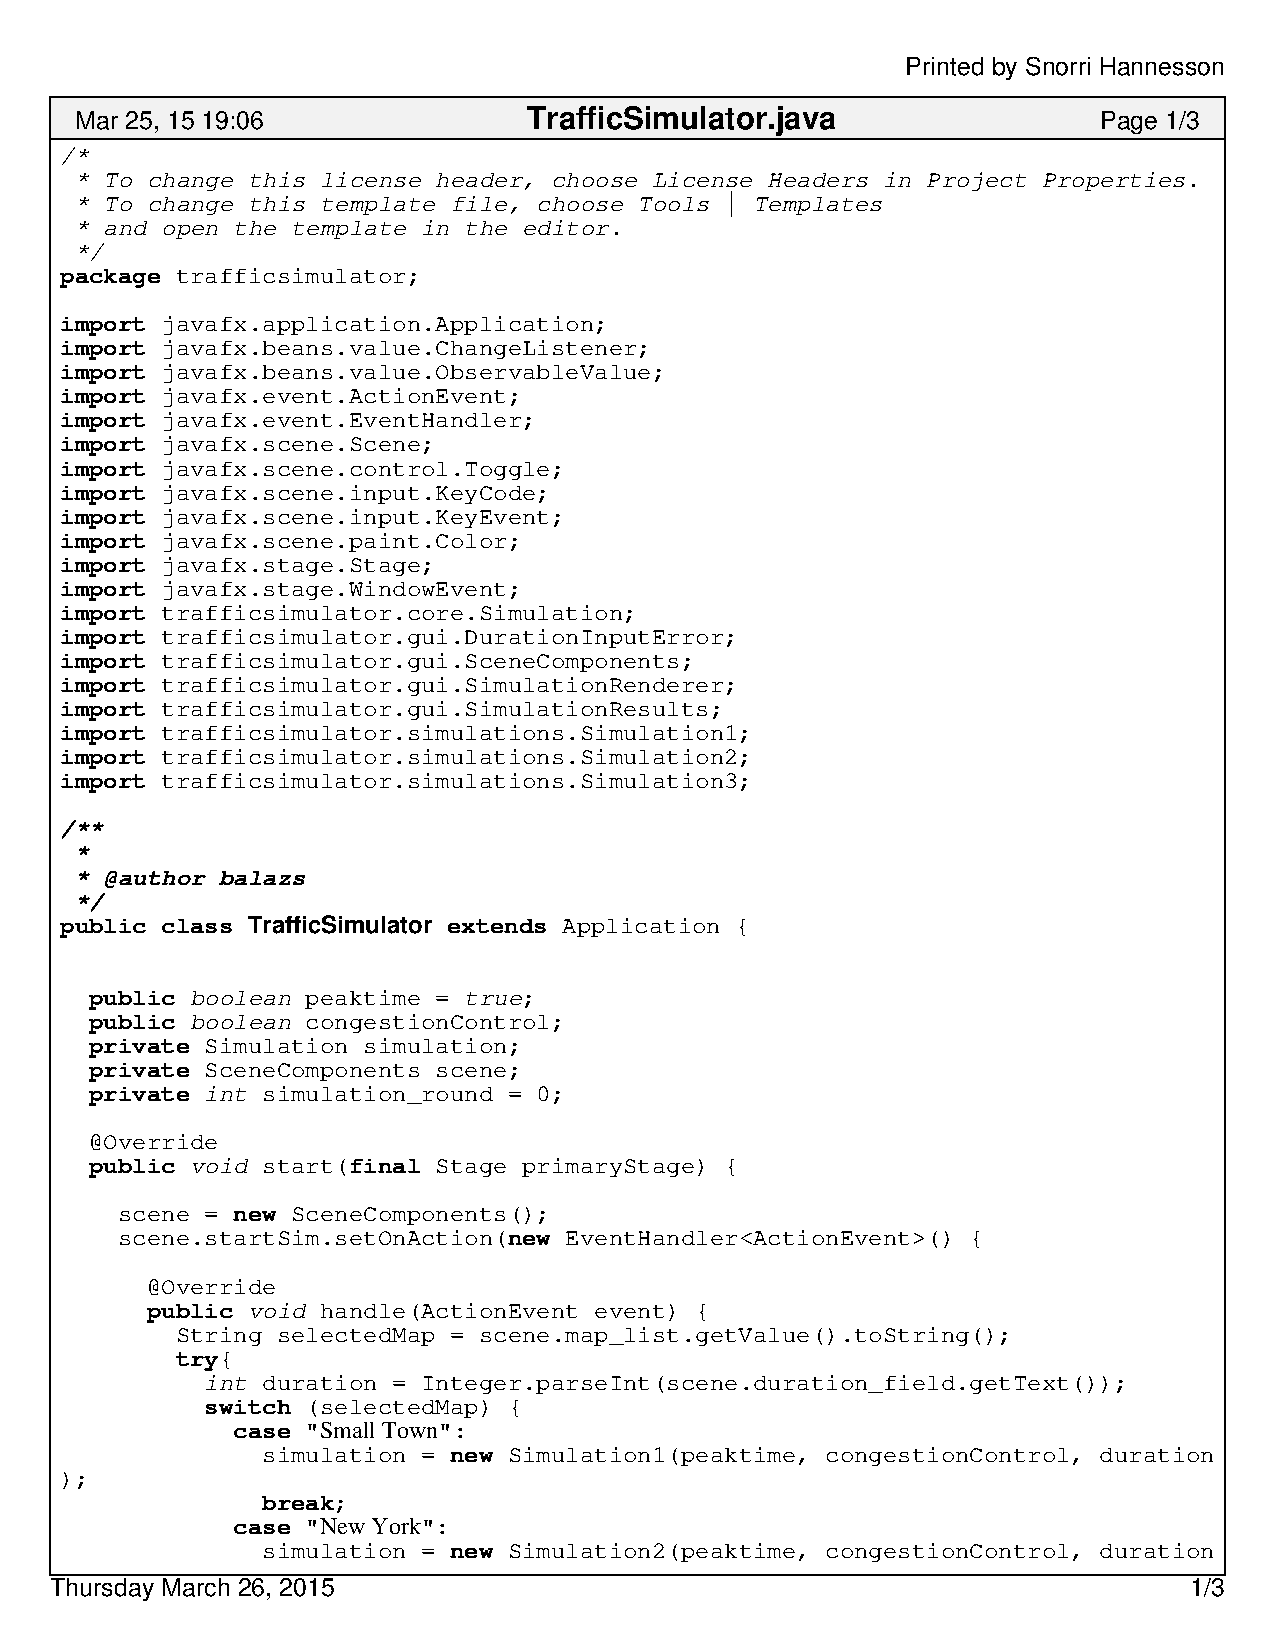
\includepdf[pages=-]{Appendices/code/sim.pdf}
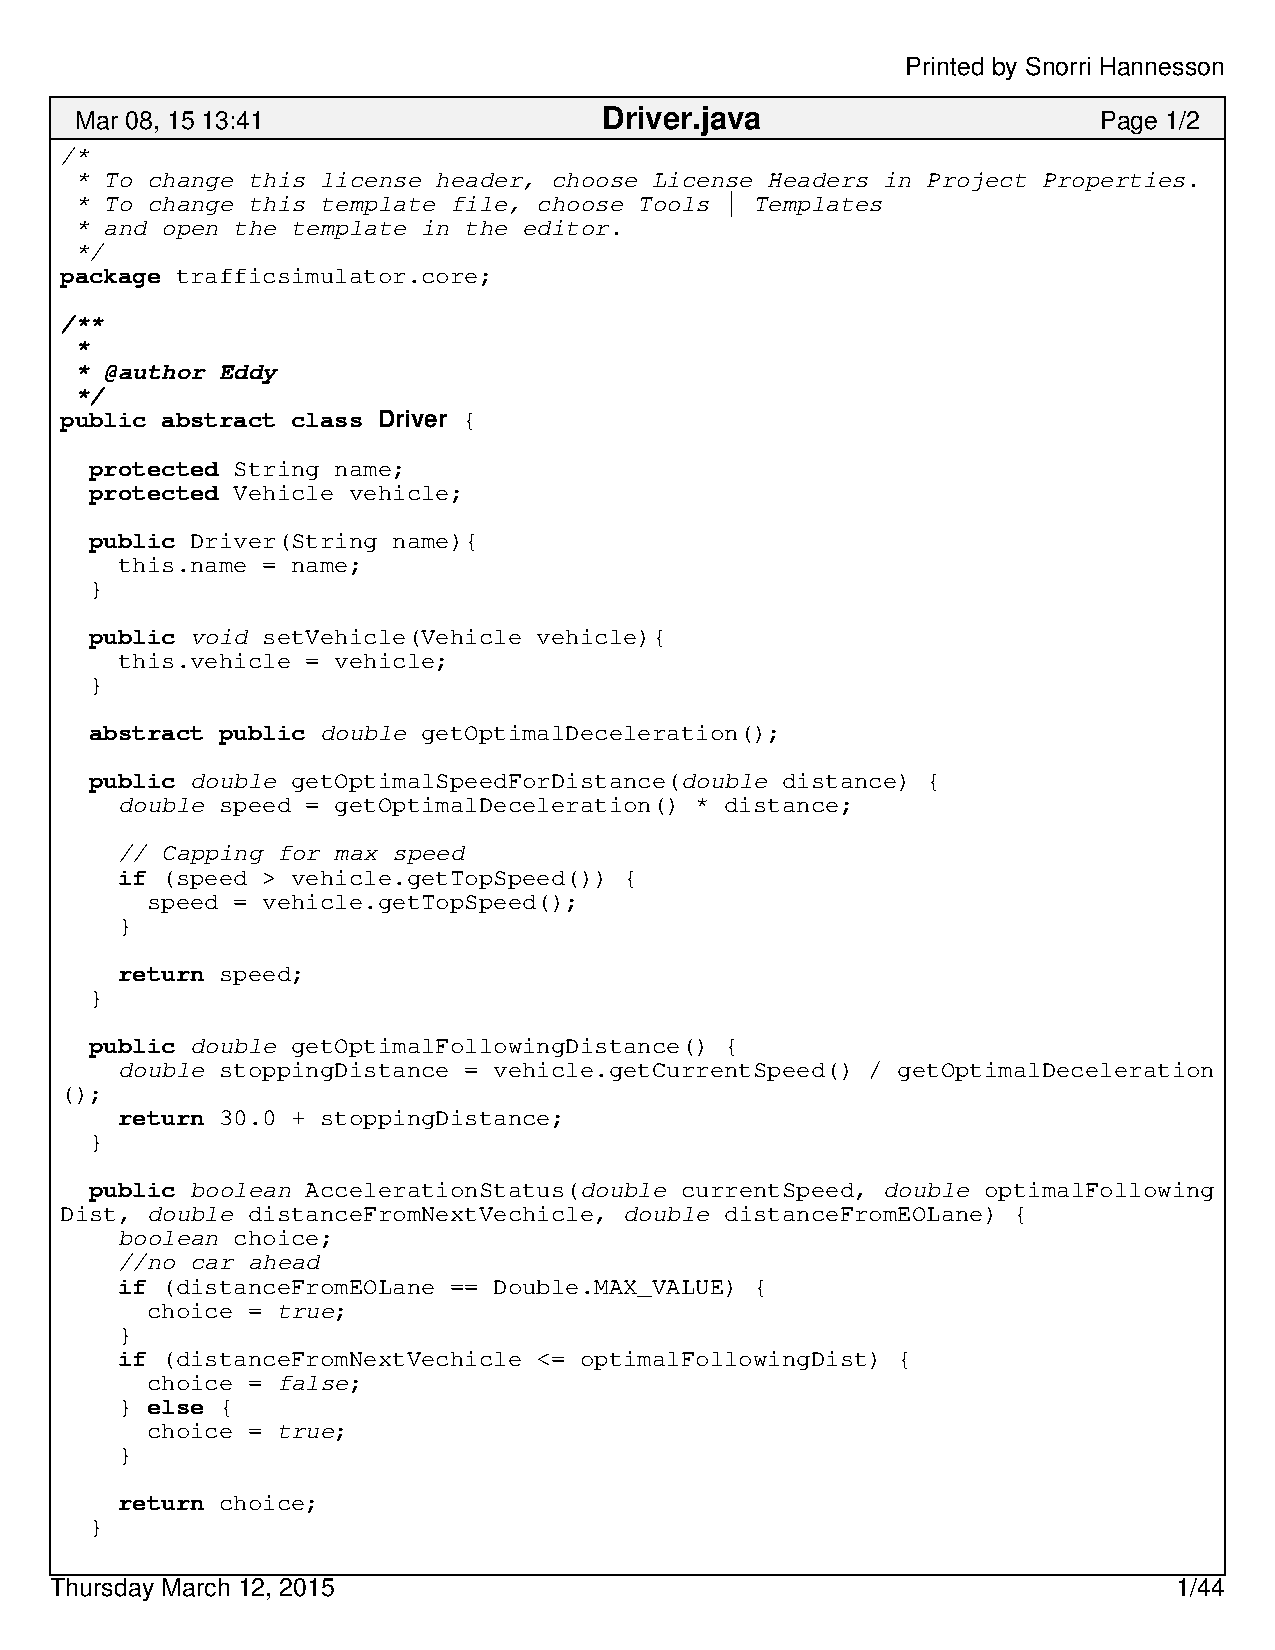
\includepdf[pages=-]{Appendices/code/core.pdf}
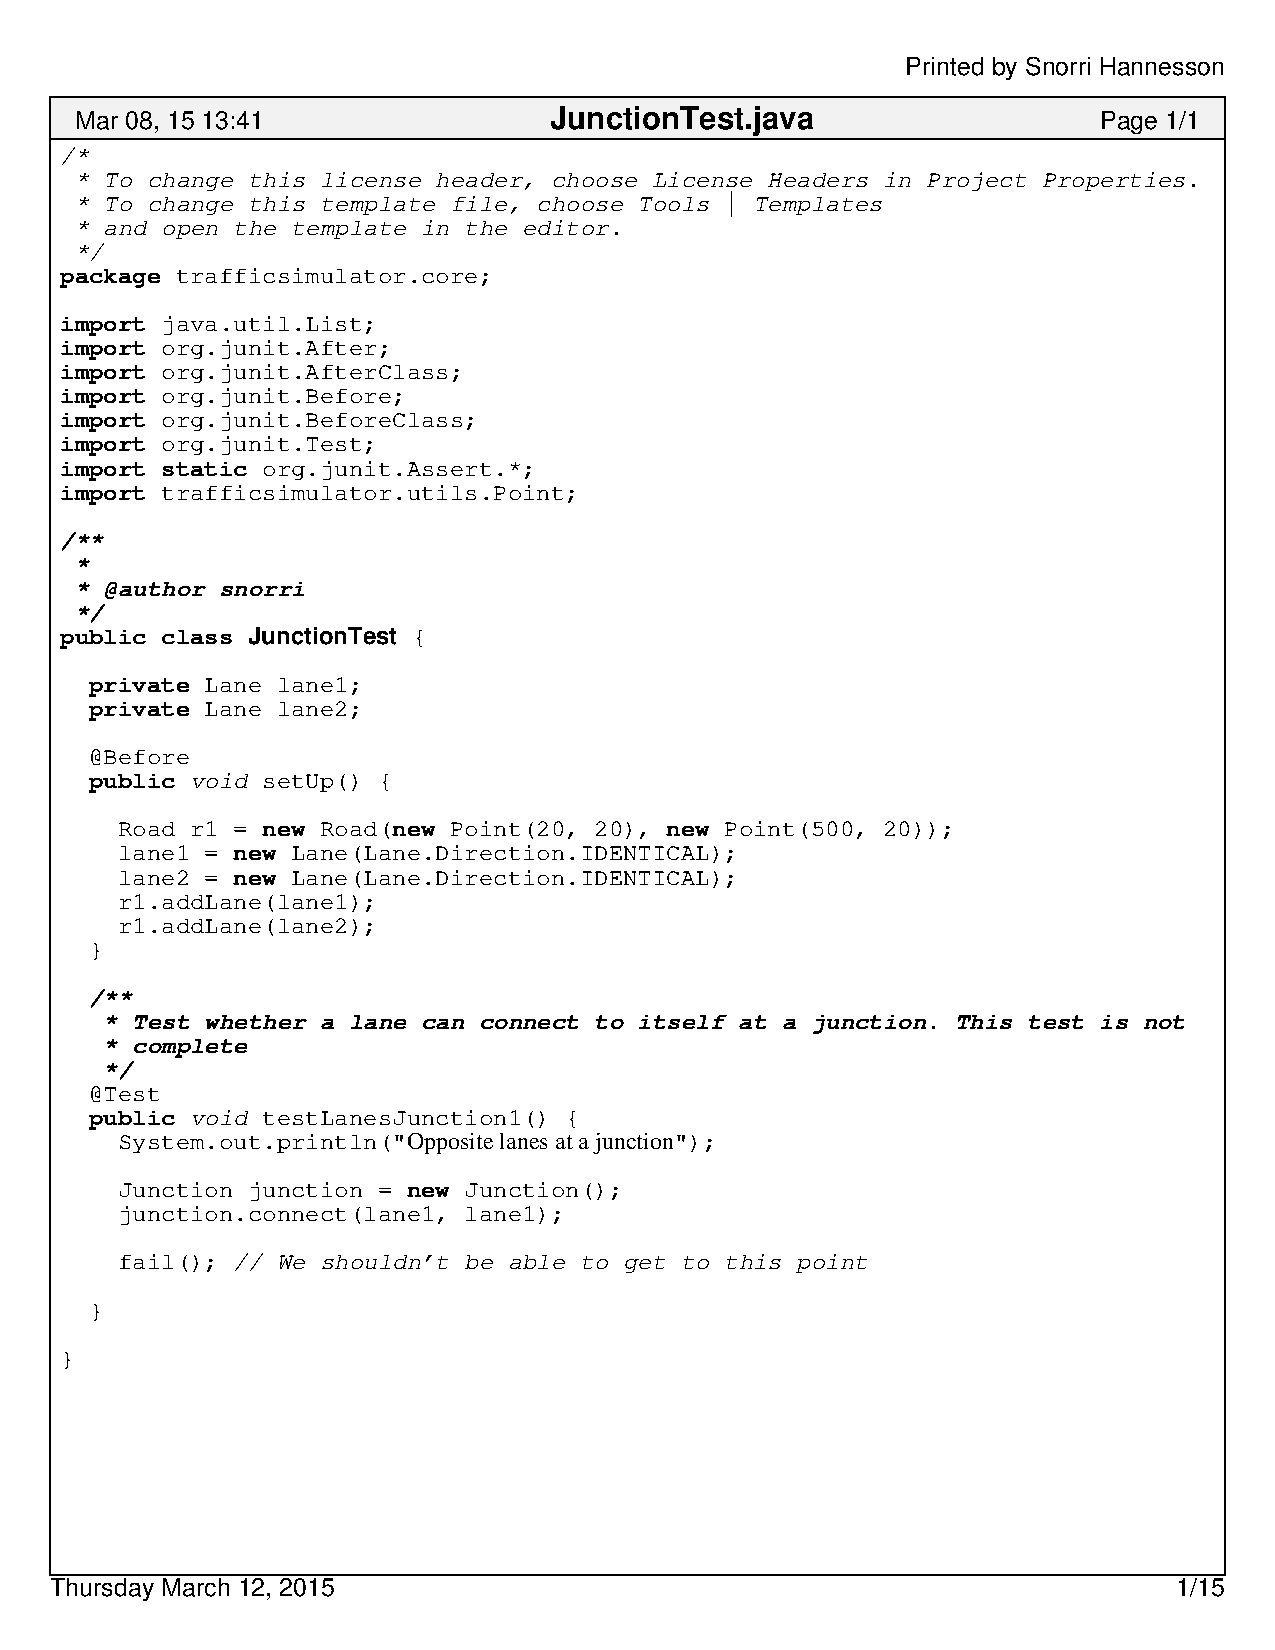
\includepdf[pages=-]{Appendices/code/tests.pdf}

\newpage	
%----------------------------------------------------------------------------------------
%	This is the initial report:
%----------------------------------------------------------------------------------------

\textbf{Project description}


\textbf{Background}
Over the past few decades, the world's population has been continuously increasing. This increase in population has resulted in overwhelming traffic which is becoming a serious problem in most major cities around the world. Cities like London, Bangkok, and New York are faced with serious traffic congestion challenges. To be able to handle these challenges and make the traffic run smoother many different traffic management policies have been tried. Before these policies can be implemented in the real world they are tested on traffic simulators. These simulator are supposed to be abstract models of the real world, so if a traffic management policy works on the simulator it probably works in the real world. In this module we will develop a traffic simulator.


\textbf{Objectives}
\begin{itemize}
\item[•] To develop a traffic simulator program which has the following structure: two types of vehicles, three types of drivers, functional road system with many roads and lanes, junctions, intersections and traffic lights.
\item[•] To compare two different traffic management policies: Fixed Time Policy and Congestion Control Policy.
\item[•] To examine how the system reacts in a time of emergency by injecting an ambulance to the simulator.
\end{itemize}

\textbf{Scale}
\begin{itemize}
\item[•] Each road can have multiple lanes, which can be in the same or opposite direction.
\item[•] As in Britain the traffic is left-lane oriented.
\item[•] The system will have cars and buses.
\item[•] Driver behaviour can be cautious, reckless, or normal.
\end{itemize}

\textbf{Outline}
\begin{description}
\item[Description]:
The traffic simulator is an abstract model of actual real world traffic. The simulator will have both cars and buses. Drivers' behaviour can be cautious, reckless or normal. Two different traffic management policies will be implemented witch are supposed to relief traffic congestion issues. The two policies are fixed time policy and congestion control policy. These policies can be compared by average time each vehicle is in the system. Moreover, an emergency strategy will be implemented to see how the system reacts when an ambulance is injected to the system. 
\newline
The simulator will be programmed in Java programming language. The simulator will have a graphical user interface (GUI). The GUI is created with the help of JavaFX software platform. The rational for using a GUI: 1. Better visualisation and understanding of code during development, i.e. actually seeing what is happening when programming collision detection. 2. When the final product is ready users can see the road system and the cars and therefore get a better understanding of how the road system is and how the policies work. Opposed to just get the result log and results of which policy is superior and have no visual understanding of what happened. 
\item[General Concept]:
	\begin{itemize}
		\item[1. ]\underline{Vehicle Types}: There are two types of vehicles: cars and buses. Cars go faster and have higher acceleration than buses. The shape and size of the bus is bigger than car, so it takes more space on the road.
		
		\item[2. ] \underline{Driver Behaviour}: The drivers can behave in three different ways: cautious, reckless, and normal. Reckless drivers drive faster than normal but the cautious drivers drive slower than normal. Reckless drivers are more prone to change lanes and overtake other vehicles, if a fast vehicle is stuck behind a slow vehicle the fast vehicle will try to overtake the slow vehicle.

		\item[3. ] \underline{Emergency Strategy}: When an ambulance is injected to the system it gets highest priority. That means that cars on the right lane will change to the left lane if possible to free the right lane for the ambulance. Also, the ambulance gets to pass at the intersection first.

		\item[4. ] \underline{Traffic Management Policy}: There are two different traffic management policies; \textit{Fixed Time policy} and \textit{Congestion Control policy}:

		\begin{description}
		\item The \textbf{Fixed Time Policy} will have peak hours (when the traffic density is the highest) and off-peak hours (when the traffic density is normal). On peak hours will the duration of the green light be longer than on off-peak hours.
		\item The \textbf{Congestion Control Policy} will always have the same duration of green light in each direction unless the system detects a congestion. When a congestion is detected in some direction the duration of the green light will be increased in that direction for one time to avoid traffic jam. \\
		\end{description}
		
The two different policies will be compared by average time each vehicle is in the system. Each vehicle will have a timer that starts when it enters the system and gets written to a log when the vehicle exits the system. The average time that a vehicle is in the system is calculated and the the policy that generates lower average time is considered better.
		 		
		
	\end{itemize}
\end{description}

\textbf{Schedule}

The time period is divided into three iterations and then the tasks allocated to the iterations. Each task is either mandatory or optional for the simulator:

\begin{table}[h]
\begin{tabular}{
>{\columncolor[HTML]{9B9B9B}}l 
>{\columncolor[HTML]{32CB00}}l 
>{\columncolor[HTML]{32CB00}}l 
>{\columncolor[HTML]{C0C0C0}}l 
>{\columncolor[HTML]{C0C0C0}}l 
>{\columncolor[HTML]{3166FF}}l 
>{\columncolor[HTML]{C0C0C0}}l }
\cellcolor[HTML]{FFFFFF}                                                                    & \multicolumn{4}{c}{\cellcolor[HTML]{FFFFFF}{\color[HTML]{32CB00} Mandatory}}                                                                                                                                                                                                                                              & \multicolumn{2}{c}{\cellcolor[HTML]{FFFFFF}{\color[HTML]{3166FF} Optional}}                                                                                                \\
\begin{tabular}[c]{@{}l@{}}\textbf{Iteration 1:}\\ 16th of January -\\ 12th of February\end{tabular} & Roads                                                                   & Lanes                                                    & \cellcolor[HTML]{32CB00}\begin{tabular}[c]{@{}l@{}}Multiple\\ vehicles\end{tabular} & \cellcolor[HTML]{32CB00}\begin{tabular}[c]{@{}l@{}}Different\\ driver\\ behaviour\end{tabular} & \cellcolor[HTML]{C0C0C0}                                                            &                                                                                      \\
\begin{tabular}[c]{@{}l@{}}\textbf{Iteration 2:}\\ 13th of February -\\ 5th of March\end{tabular}    & \begin{tabular}[c]{@{}l@{}}Junctions\\ and\\ intersections\end{tabular} & \begin{tabular}[c]{@{}l@{}}Traffic\\ lights\end{tabular} &                                                                                     &                                                                                                & \begin{tabular}[c]{@{}l@{}}Different\\ traffic\\ management\\ policies\end{tabular} &                                                                                      \\
\begin{tabular}[c]{@{}l@{}}\textbf{Iteration 3:}\\ 6th of March -\\ 26th of March\end{tabular}       & \cellcolor[HTML]{C0C0C0}                                                & \cellcolor[HTML]{C0C0C0}                                 &                                                                                     &                                                                                                & \begin{tabular}[c]{@{}l@{}}Time\\ logging\end{tabular}                              & \cellcolor[HTML]{3166FF}\begin{tabular}[c]{@{}l@{}}Emergency\\ Strategy\end{tabular}
\end{tabular}
\end{table}


\textbf{Expectation of Project Outcome}
\begin{itemize}
\item[•] The traffic simulator is developed and implemented.
\item[•] Results showing which traffic management policy is superior or if they are equal.
\item[•] The simulator can be used in case of emergency.
 
\end{itemize}

\textbf{Current progress}
We are currently finished with iteration 1 and we are on schedule. We have implemented the roads, lanes that can go in the same or opposite direction, different vehicles and different drivers' behaviour. However, we are still trying to find the best architecture for the different drivers' behaviour and vehicles. \\
As the name of the team implies; we are a very diversified group. From four different countries in three different continents, each with different programming background and experience. Although some of the members of the team were familiar with git and GitHub, LaTeX and some of the other technical tools we are using, some team members weren't. For everyone in the team to be able to make an contribution we have spent a quite a lot of time discussing those technical tools. \\
The biggest challenge so far is to get everyone on the same page about the project and the tools used for developing and collaboration.


%----------------------------------------------------------------------------------------
%	PART TWO
%----------------------------------------------------------------------------------------

\textbf{Project organisation}
\textbf{Project management}
A slightly adjusted Agile Methodology is used for this project. We have divided the time period for this course into iterations and at the end of each iteration we want to be inching forward towards the final product.

\textbf{Roles}


\textbf{Balázs Kiss:} Lead programmer \\
\textbf{Eddy Mukasa:} Architect \\
\textbf{Yukolthep Visessmit:} Graphical designer \\
\textbf{Pongsakorn N. Riyamongkol:} Project Manager \\
\textbf{Snorri Hannesson:} Tester and Coordinator \\ \newline
Each member of the group has a responsibility to oversee one aspect of the project but is not expected to do all the work defined in his role. I.e. each member should/could do some programming but the lead programmer should oversee the code and make sure nothing is missing and everything is done properly. The same goes for the other roles.

\textbf{Collaboration}
We have physical meeting every Thursday at 10 o'clock. We have a log of all meetings. Other means of collaborations are:
\newline \\
\textbf{Facebook} is used as a communication channel. \\
\textbf{GitHub} is used for version control. \\
\textbf{Trello} is used for project management.


\textbf{Peer Assessment and Self Assessment}
Team members should evaluate their own and other members' performance regarding work done in the group. This can be
done by using an assessment form where every member secretly grades themselves and other members of the team. Then can contributions to
\textbf{GitHub} and \textbf{Trello} be examined for evaluation of members performance.

\textbf{Conflicts}
If we have a conflict during this project the will have democracy; the majority decides. However, if a major conflict arises we will have to contact the instructor to resolve the conflict. We have defined a simple method to resolve conflicts: 
\newline
\textbf{I.} Realise conflict. \\
\textbf{II.} Handle conflict sooner rather than later. \\
\textbf{III.} Find the solution together - democracy. \\
\textbf{IV.} Apologise. \\
\textbf{V.} Appreciate. \\
\end{document}